%!TEX root = ../Studienarbeit.tex

\section{Bilderkennung und -Verarbeitung}

\subsection{Object Detection}

\subsubsection{Training}

\subsubsection{Deployment}

\subsection{Benchmarks}

\subsection{Erkennung durch Kontur-tracking}

\subsection{Verbesserung der Bildqualität}

\subsection{Tiefenberechnung}


\section{Hardwarerealisierung}

Für einen optimalen Vertreibungseffekt werden verschiedene Aktoren im System verbaut. Die einzelnen Geräte werden alle über eine externe Energieversorgung, beziehungsweise Batterie betrieben. Bei der Wahl der Batterie, ist ein wichtiges Kriterium, wie lange das System ohne Energiezufuhr funktionsfähig bleibt.
\\
Dabei wurde berücksichtigt, wie viel das System im Normalverbrauch ohne Einschalten der Aktoren verbraucht. Eine grobe Schätzung ergab, dass das System ungefähr 10 $\pm$ 2 Watt pro Stunde verbrauchen würde. Aus diesem Grund fiel die Wahl auf eine 50 Ah Autobatterie von \textit{BlackMax} \cite{Autobatterie} gefallen. Diese Batterie bietet ausreichend Kapazität, um das System über zwei Tage mit Energie zu versorgen.
\\
Ein weiterer Entscheidungsgrund für die Autobatterie ist der Strombedarf der Geräte. Wie nachfolgend beschrieben, kann die Wasserpumpe im laufenden Zustand bis zu 16 Ampere Strom beziehen. Viele leichte und kleine Batterien könnten langfristig durch diese Belastung Schaden nehmen. Da Autobatterien eine hohe Belastungsgrenze haben und hohe Ströme ermöglichen, sind sie daher für den Prototypen besser geeignet.

Für die Unterbringung aller Teile wird eine 40x55x30 cm große Aluminiumkiste verwendet. Die Aluminiumkiste ist witterungsbeständig, und die Wärmeentwicklung im Inneren kann weitestgehend vernachlässigt werden. Aluminium hat nämlich eine gute Temperaturleitfähigkeit und kann somit einen Wärmestau verhindern. Dabei ist auch der Empfehlung aus einem \textit{Autodesk Instructables}-Projekt folge geleistet worden. In diesem Projekt wurde eine bewegungsausgelöste "`Wasserpistole"' aufgebaut. Allerdings war bei dem \textit{Instructables}-Projekt eine Vertreibung von Rehen vorgesehen, die sonst die Rosen im Garten aufgegessen hätten. Das Ziel dieser Arbeit ist es aber Waschbären und andere Kleintiere zu vertreiben, daher sind hier noch weitere Aktoren eingebaut. Zudem ist das \textit{Instructables}-Projekt nicht autark und portable, da es mit Strom und Wasser mittels Hausanschluss versorgt worden ist. \cite{watergun_dude}

Die eingebauten Bauteile werden nachfolgend beschrieben.

\subsection{Blitzlicht}

Für den Einsatz eines Abschrecklichtes mit Blitzlichtfunktion werden zwei LED-Scheinwerfer der Marke \textit{NAIZY} verwendet. Die Scheinwerfer sind für den Einsatz als Erweiterungsleuchten für Geländefahrzeuge gedacht. Sie sind wasserdicht und für den Außeneinsatz geeignet. Mit 1600 Lumen und grellweißem Farbton erzielen sie einen hohen stroboskopischen Effekt, mit dem die Tiere abgeschreckt werden. Aufgrund dieser Charakteristiken und des geringen Energieverbrauchs von 18 Watt sind sie für das Abschrecksystem sehr gut geeignet. \cite{am_licht}

Die beiden LED-Scheinwerfer sind an den beiden oberen Ecken der Box befestigt. Sie werden mit Transistoren durch den Mikrocontroller gesteuert. Um einen Gewöhnungseffekt zu vermeiden, sind die Scheinwerfer mit 0,5 bis 10 Hz beschaltet. Die Frequenz und Schaltung der Scheinwerfer wird dynamisch angepasst. Im Schaltbild aus Abbildung \ref{diag:lights_diagram} wird die Verwendung eines MOSFET-Treiberbausteins erkennbar. Der Treiber ermöglicht das Beschalten der Scheinwerfer mit höherer Leistung, als es mit dem Arduino möglich wäre. Der Treiber verfügt über eine zusätzliche Masse-Leitung, die mit dem Arduino verbunden ist. Dadurch ist es möglich den Strom zu schalten, auch wenn der Signalgeber und \textit{DC-Out} nicht die selbe Masse haben. \cite{mosfets_am}

\begin{figure}[h]
    \centering
    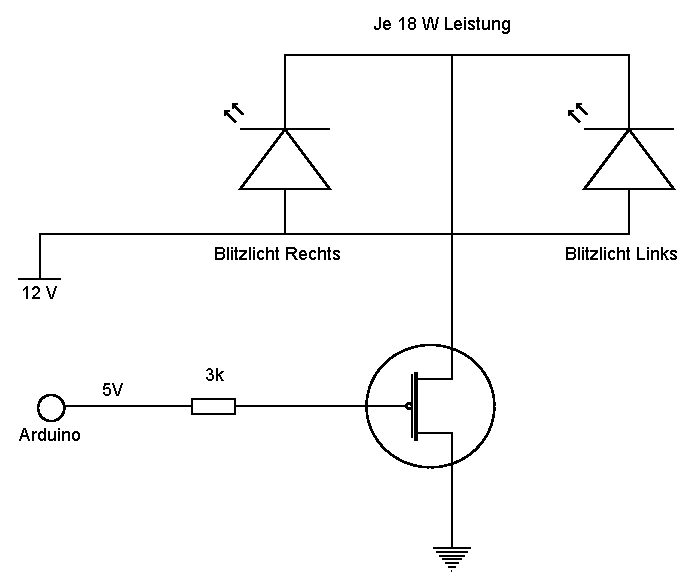
\includegraphics[width=0.6\textwidth]{images/lights_diagramm.pdf}
    \label{diag:lights_diagram}
    \caption{Schaltbild der Abschreckleuchten mit Ansteuerung}
\end{figure}

\subsection{Wasserversorgung und Pumpeneinheit}

Für den Einsatz eines \textit{Abschusssystems} mit Wasser benötigt das Abschrecksystem weitere Komponenten, welche folgend beschrieben werden.

\subsubsection{Pumpe}

Auch wenn die Aluminiumkiste witterungsbeständig ist, schützt sie nur mäßig vor kalten Temperaturen. Dabei können viele Wasserpumpen schaden nehmen, wenn sie über den Winter draußen sind. Bei Membranpumpen ist dies ein kleineres Problem. Die zu den Oszillationsverdrängerpumpen gehörende Pumpenart ist außerdem sehr wartungsfreundlich und außerordentlich robust. Sie können daher selbst schwierigen Bedingungen und Temperaturumschwünge leicht standhalten.
\\
Ihre Funktionsweise beruht darauf, den \textit{Schöpfraum} periodisch zu vergrößern und zu verkleinern. Dadurch erzielen sie ihre Pumpwirkung und werden durch ihre Robustheit, Ölfreiheit (keine Verschmutzung der zu fördernde Flüssigkeit oder Gase) und Wartungsfreundlichkeit auch in chemischen Laboranwendungen verwendet. \cite{Jousten2018}

Für die Auswahl einer geeigneten Pumpe kamen zudem die Anforderungen an Fördermenge und Druck. Sprinkleranlagen werden wie in Kapitel \ref{sprinkler} beschrieben mit einem Gartenschlauch betrieben und können mit dieser Versorgung eine Reichweite von 10 Metern erreichen. Durch einen Hausanschluss fließen üblicherweise 20 Liter Wasser pro Minute mit einem Druck von etwa 4 Bar.\\
Die eingesetzte Pumpe von \textit{SEAFLO} hat eine maximale Fördermenge von 17 Liter pro Minute und kommt dadurch nahe an diesen Richtwert ran. Dabei nimmt sie bis zu 16 Ampere Strom auf. Auch bei dieser Leistungsaufnahme von über 190 Watt können die MOSFET-Treiber, die zum An- und Ausschalten der LED-Scheinwerfer verwendet werden, genutzt werden. Sie sind angegeben mit einer Dauerbelastung von 15 Ampere und mit Kühlung bis zu 30 Ampere. Da die Treiber nur für kurze Dauer eingeschaltet werden, ist eine zusätzliche Kühlung nicht nötig. \cite{mosfets_am,seaflo_pump}

Der Aufbau ist ähnlich zu dem Schaltbild \ref{diag:lights_diagram}. Allerdings wird zusätzlich eine Schutzdiode benötigt. Da Pumpen durch den internen Betrieb mittels Elektromotor eine induktive Last bilden, kann bei hartem Ein- und Ausschalten der MOSFET-Treiber durch Spannungsstöße Schaden nehmen \cite{induktive_last_diode}. Daher wird eine Schottky-Diode parallel zur Last eingebaut. Dies verhindert ein Aufbauen zu hoher Spannung, durch der der Transistor Schaden nehmen könnte. Schottky-Dioden eignen sich besonders gut für den Einsatz, da sie nur wenig Leistung aufnehmen und dadurch energiesparend sind. \cite{induktive_last_diode,am_schottky}

\subsubsection{Versorgung mit Wasser}

Damit die Pumpe mit Wasser versorgt werden kann, muss ein Wassertank in das System integriert sein. Allerdings ergeben sich dadurch verschiedene Probleme.
\\
Das größte Problem, das gelöst werden muss, ist die Unterbringung des Wassertanks. Durch den Einbau der verschiedenen Aktoren sowie der Autobatterie wurde in der Aluminiumkiste bereits viel Platz verwendet. Ein speziell an den verfügbaren Platz angepasster Tank kann zudem nicht mittels 3D-Drucker hergestellt werden, da die Drucke nicht wasserdicht sind. Ein herkömmlicher und einbaubarer Wassertank könnte daher nur wenige Liter fassen.

Ein weiteres Problem betrifft die Dichtigkeit des Tanks und der Pumpe. Beim Transport der Aluminiumkiste könnte eine große Menge Wasser leicht austreten. Aufgrund der Leitfähigkeit des Wassers könnten die Elektronikkomponenten Schaden nehmen. Dies wäre jedoch nicht so gravierend, da die Elektronik lediglich durchbrennen und der Stromkreislauf unterbrochen würde. Allerdings besteht bei der Aluminiumkiste die Gefahr, dass sie vollständig unter Strom gestellt wird. Dadurch würde sogar eine potenzielle Lebensgefahr entstehen, wenn man die Kiste berührt.
\\
Um die Sicherheit zu erhöhen, wird der Wassertank deshalb außerhalb der Kiste platziert und der Zulauf erfolgt durch eine seitliche Öffnung an der Kiste. Die Pumpe befindet sich jedoch weiterhin innerhalb der Kiste, um sie vor den äußeren Witterungsbedingungen zu schützen. Sie wird durch einen gedruckten Spritzschutz räumlich von den anderen Aktoren und der Spannungsversorgung getrennt. Der 3D-Druck ermöglicht jedoch keinen vollständigen Schutz, da er nur gegen geringe Wassermengen dicht hält. Spritzwasser und kleinere Leckagen durch die Pumpe können jedoch bewältigt werden.
\\
Vor dem Einbau in die Kiste wurde ein Dichtigkeitstest der Pumpe und des Spritzschutzes durchgeführt. Dabei traten nur bei bestimmten Bedingungen, wie dem seitlichen Legen oder Schütteln der Pumpe, geringe Mengen Wasser aus der Pumpe aus. Daher sollte der gedruckte Spritzschutz einen ausreichenden Schutz bieten.

\subsection{Mikrocontroller}

\subsection{Sensorik-Kameras}

\subsection{Ansteuerung}

mosfet -> bei 3.3V runterregeln des Stroms

\comment{Verkabelung, Aufbau, Herausforderungen, spezielle Lösungen}
Auswahl PI -> Liefermangel
Erstidee Multiplexer um zeitverzögerung zu reduzieren -> schlechte Kritik
% https://www.amazon.de/Arducam-Adaptermodul-Raspberry-kompatibel-Kameras/dp/B07TYL36MC/ref=sr_1_5?__mk_de_DE=%C3%85M%C3%85%C5%BD%C3%95%C3%91&crid=2KI1QVYFS8KN6&keywords=camera+adapter+raspberry&qid=1662198136&sprefix=camera+adapetr+raspberry%2Caps%2C77&sr=8-5

Zweite Idee usb-> von vornerein "komplexer" /durch zeitkacke -> irgendwie auch teuer

Dritte Idee esp32-CAM Module -> Hohe Latenzen und Zeitsynchronitätsaufwand

Viertens -> compute model + I/O shield auch teuer aber 2 csi Anschlüsse

5. Jetson mit 2 CSI Anschlüssen -> teuer und noch mehr Liefermangel

\subsection{Wasserversorgung}

integrierte Pumpe $\rightarrow$ Soll portable sein

Alternativ: Gartenschlauch mit Ventilsteuerung



\section{Dreidimensionales Zielsystem} \label{cap:dreidim}

\begin{wrapfigure}{l}{0.4\textwidth}
    \centering
    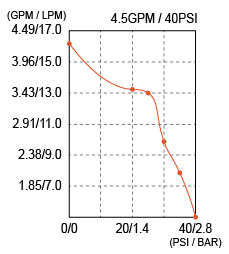
\includegraphics[width=0.35\textwidth]{images/seaflo_lpm_psi.png}
    \label{fig:psi_seaflo}
    \caption{Diagramm der Fördermenge gegenüber des Drucks. \cite{seaflo_pump}}
\end{wrapfigure}
Aus dem Diagramm in \ref{fig:psi_seaflo} ist zu entnehmen, das die Pumpe eine minimale Fördermenge von 5 Litern pro Minute hat. Demnach kann die Austrittsgeschwindigkeit des Wassers berechnet werden. Hierfür wird lediglich die Fördermenge und der Querschnitt des Laufs benötigt. Die Austrittsgeschwindigkeit kann aber nicht mit der allgemeinen Gleichung $ Geschwindigkeit = \frac{Volumenstrom}{Strömungsquerschnitt}
$ aus \cite{stroemungen} entnommen werden. 
Wenn man mit der niedrigsten Fördermenge von knappen 5 Liter pro Minute rechnet, hätte man demnach eine Austrittsgeschwindigkeit von mehr als 265 Meter pro Sekunde erreicht.
$\rightarrow$ Entscheidung Servo/DC?

\comment{Mit Vision Schwerpunkt der Arbeit teils/ganz in HW-Realisierung?}

\section{Kostenaufstellung}

\begin{longtable}{ p{0.15\textwidth}|p{0.2\textwidth}|p{0.5\textwidth} }
    \endfirsthead
    \multicolumn{2}{l}%
    {\textit{Fortsetzung von vorheriger Seite}} \\
    \hline
    \endhead
    \hline \multicolumn{2}{r}{\textit{Fortsetzung auf nachfolgender Seite}} \\
    \endfoot
    \endlastfoot
    \textbf{Bauteil} & \textbf{Gesamtpreis in € (inkl. Mwst.)} & \textbf{Beschreibung}\\
    \hline
    LED-Scheinwerfer
    & \centering11.99
    & Die effizienten LED-Scheinwerfer sind für die Anwendung als Erweiterungsleuchten für das Fahrzeug gedacht. \cite{am_licht} Da die LEDs den hohen Belastungen beim Einsatz am Fahrzeug standhält, werden sie den Anforderungen an einem portablem Abschrecksystem gerecht. Sie werden als Blitzlicht für das Abschrecksystem verwendet.
    \\
    Membran-pumpe
    & \centering73.35
    & Membranpumpen sind bei einfachen und kostengünstigen Anwendungen vertreten. Durch den geringen Verschleiß und einfache Wartbarkeit werden sie häufig in Frisch- und Abwasseranwendungen eingesetzt. \cite{mebranpumpe} In der Arbeit wird die Pumpe wegen ihrem geringen Verschleißes und Anschaffungskosten verwendet.
    \\
    Solarpanel
    & \centering69.99
    & Das Solarmodul wird verwendet um die Portabilität und Autarken Eigenschaften der Abschrecksystems zu gewährleisten. Solange Sonnenlicht am Einsatzort verfügbar ist, kann das Abschrecksystem mit ausreichend Energie versorgt werden um die unliebsamen Kleintiere zu erkennen.
    \\
    Autobatterie
    & \centering59.90
    & Kombiniert mit dem Solarmodul versorgt die Batterie das Abschrecksystem mit der nötigen Energie. Tagsüber wird sie mithilfe des Solarmoduls aufgeladen, während sie Nachts das System mit Energie versorgt. \cite{Autobatterie}
    \\
    Diverse Kleinteile
    & \centering{25 + X}
    & Diverse Kleinsteile werden in der Arbeit verwendet. Auch die Transistoren, die verwendet werden um die verschiedenen Aktoren an- und auszuschalten fallen unter dieser Kategorie. Aber auch die Räder, Schläuche, Kabel, Steckverbindungen und Schrauben werden hier miteinberechnet. Zusätzlich kommen die, für das Abschrecksystem angefertigten 3D-gedruckten Elemente hinzu.
    \\
    Aluminium-kiste
    & \centering{109 DM}
    & Die Aluminiumkiste ist Witterungsfest und besitzt eine gute Wärmeableitung. Alle Aktoren und Gerätschaften können in ihr vor Witterungsbedingungen geschützt untergebracht werden.
\end{longtable}

\begin{figure}
    \centering
    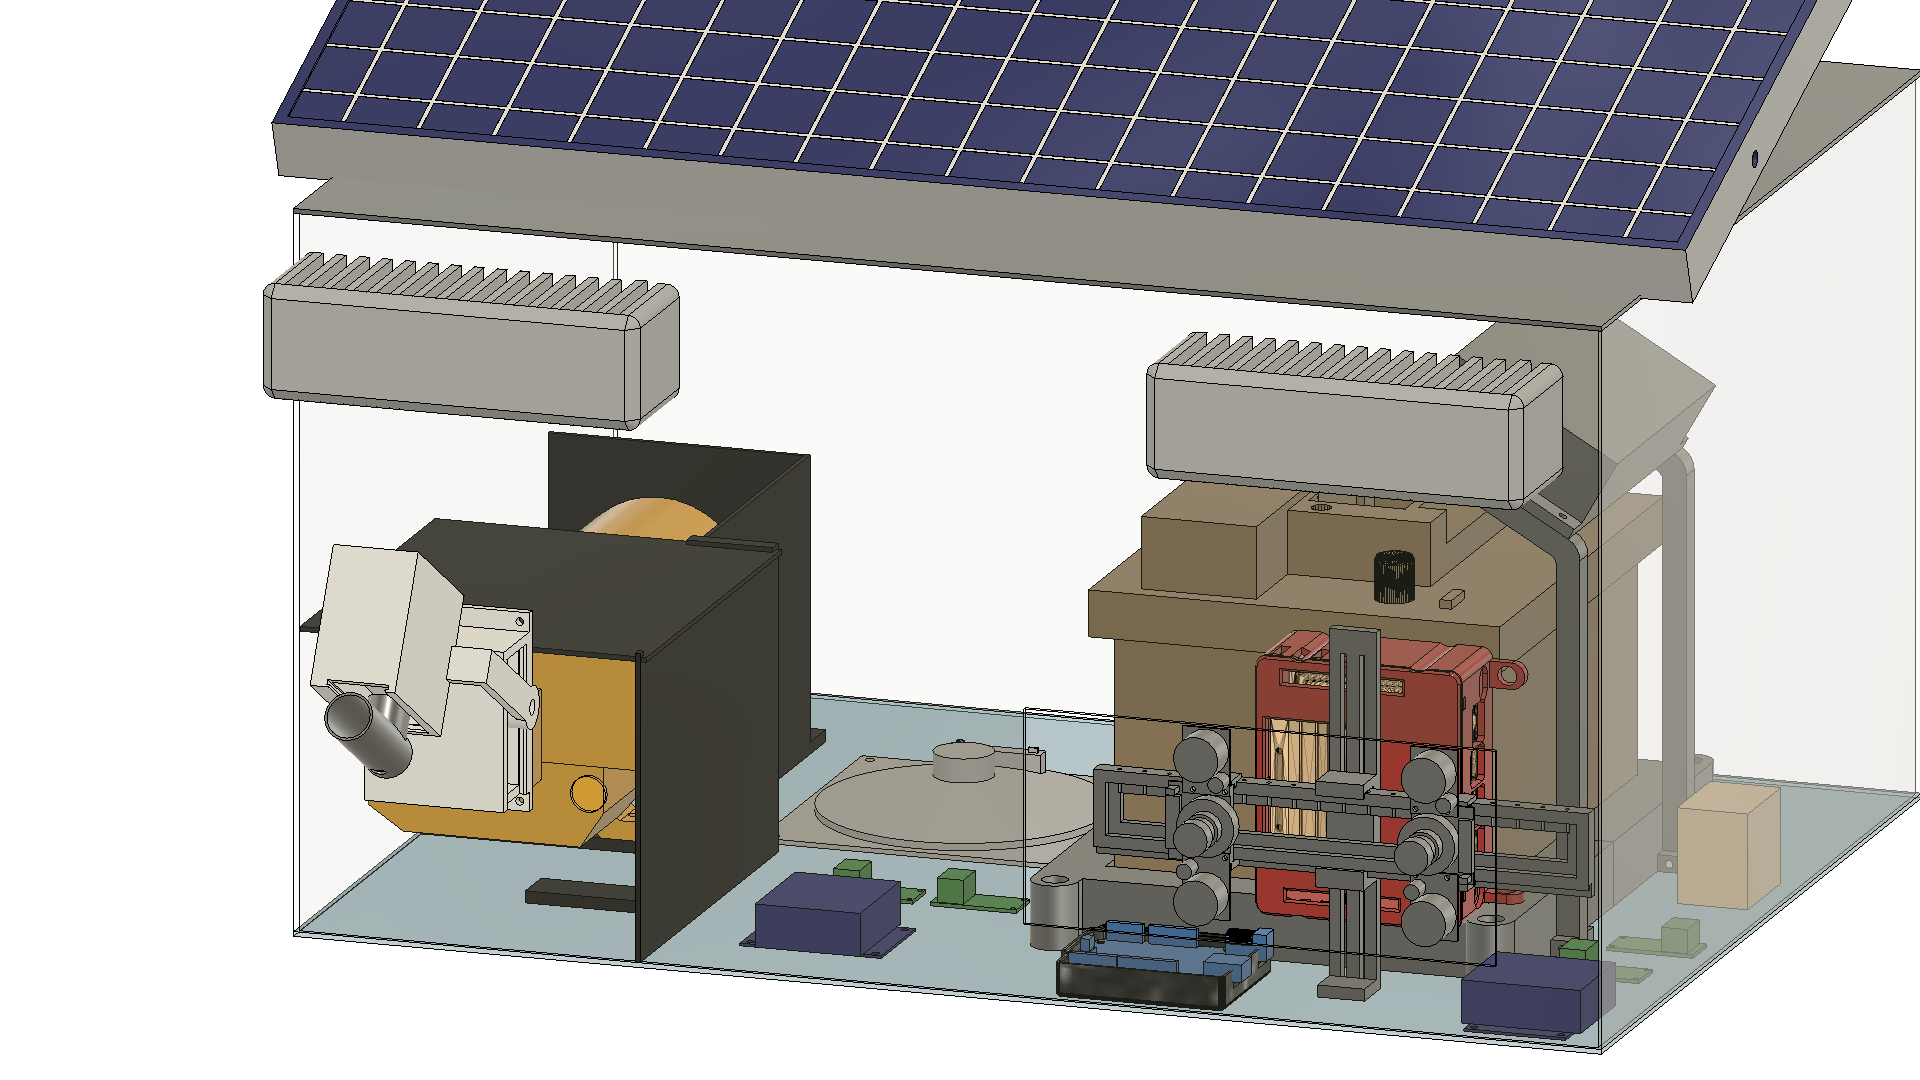
\includegraphics[width=\textwidth]{images/whole_box.png}
    \label{fig:whole_thing}
\end{figure}
